\documentclass[12pt]{article}
\usepackage[top=1.0in, bottom=1.0in, left=1.0in, right=1.0in]{geometry}
%\usepackage[ascii]{inputenc}
%\usepackage[T1]{fontenc}
%\usepackage[english]{babel}
%\usepackage{amsmath}
%\usepackage{amssymb,amsfonts,textcomp}
%\usepackage{array}
%\linespread{2}
\usepackage{graphicx}
\usepackage{amsmath, amsthm, amssymb}
\usepackage{amssymb}
\usepackage{graphics}
\usepackage{mathrsfs}
\usepackage{setspace}
\usepackage{graphicx}
\usepackage{epstopdf}
\usepackage{subfigure}
\usepackage{rotating}
\usepackage{longtable}
\usepackage{tabularx}
\usepackage{tabulary}
\usepackage{ltxtable}
\newtheorem{lemma}{Lemma}
\newtheorem{prop}{Proposition}
\newtheorem{cor}{Corollary}\newcommand{\dspace}{\renewcommand{\baselinestretch}{1.5}\small\normalsize}
\newcommand{\sspace}{\renewcommand{\baselinestretch}{1.0}\small\normalsize}

\title{\textbf{Hybrid Recommender System \\Using Artificial Neural Networks}}

\author{\textbf{Tulasi Paradarami}\\Department of Predictive Analytics\\School of Professional Studies\\Northwestern University}

\date{}

\begin{document}
\maketitle
\normalsize

\section*{Abstract}

[TBD]

\section*{Key Words}

Information Retrieval, Artificial Neural Networks, Recommender Systems, Supervised Learning

\newpage\section{Introduction}

Information overload occurs when the amount of input to a system exceeds its processing capacity. Decision makers have fairly limited cognitive processing capability. Consequently, when information overload occurs, it is likely that a reduction in decision quality will occur Speicer et al., (1999) \cite{speier}, Milord et al., (1977) \cite{milord}, Miller (1956) \cite{miller g. a. 1956.txt}, Simon (1979) \cite{simon h. a. 1979.txt}. When a large amount of data is available in a variety of formats and reaching at a rate too high for the user to efficiently process, it leads to information overload (Edmunds and Morris, 2000) \cite{edmunds}. In the current era of smart devices and Web 2.0, there is a massive amount of data generated from a wide variety of sources including but not limited to social networking sites, multimedia sharing sites, hosted services, email, group communications, instant messages. It is getting harder for users to find relevant content on the web and on many occasions this information overload can cause users responding to the problem by omitting something important or making an error in the process of making a decision (Vickery and Vickery, 2004) \cite{vickery}. Whether it is for personal or professional needs, users cannot ignore the information available to them but need intelligent techniques that can efficiently filter the data and present most relevant information.

A Recommender System (RS) is an application that is built to cope with the problem of information overload and provide intelligent suggestions on items to users (Ricci et al., 2011) \cite{ricci}, (Recommender Systems.html) \cite{recommender systems.html}. This ability of a RS to provide an efficient means to find relevant items is extremely useful because of which RS have become an important research area that has attracted attention in both academia and industry (Adomavicius and Tuzhilin, 2005) \cite{adomavicius-2005}. In simple terms, RS generates a personalized list of ranked items for users to buy from, where rank is computed from heterogenous sources of data acquired from the user like interests, likes and dislikes, demographics (Ricci et al., 2011) \cite{ricci}. Interest in recommender systems has remained high because of the wide variety of applications that can help deal with information overload by providing personalized recommendations. Few examples of these recommendation systems are product recommendations by Amazon.com (Linden et al., 2003) \cite{linden}, movies by Netflix (Amatriain, 2013) \cite{amatriain}, news articles (Nanas et al., 2010) \cite{nanas}, financial services (Felfernig et al., 2007) \cite{felfernig}, twitter (Gupta et al., 2013) \cite{gupta}. A RS can support a variety of functions that gives reason for service providers to deploy these techniques on their infrastructure. Some of the more important functions of RS are increasing sales by selling more items, improving user experience, satisfaction and better understand users' needs (Ricci et al., 2011) \cite{ricci}

Recommender systems are broadly classified into following categories based on the underlying technique used for making recommendations (Adomavicius and Tuzhilin, 2005) \cite{adomavicius-2005}, (Burke, 2002) \cite{burke}, (Jannach et al., 2010) \cite{jannach}:

\begin{enumerate}
\item Collaborative filtering: It evaluates the relevance of an item for a user based on the opinion of the members of a community (or cluster) (Nanas et al., 2010) \cite{nanas}. It runs on the premise that users with similar interests tend to prefer similar items.
\item Content based filtering: It assumes that items with similar characteristics will be rated in a similar way (Wu et al., 2014) \cite{wu}. That is, it recommends items that are similar to the ones liked by the user in the past.
\item Knowledge based recommender systems: Such a system recommends products based on specific domain knowledge on how certain item features satisfies users' needs and specifications (Ricci et al., 2011) \cite{ricci}. 
\item Hybrid recommendation systems: Any combination two or more techniques described above can be categorized as a hybrid recommendation system (Jannach et al., 2010) \cite{jannach}.
\end{enumerate}

Artificial Neural Networks (ANNs) have a long history and research article of (McCulloch et al., 1943) \cite{mcculloch}, (Cochocki and Unbehauen, 1993) \cite{cochocki} is generally considered the beginning of Neurocomputing. After few years of calm, ANNs have started to gain popularity in 1980s (Cochocki and Unbehauen, 1993) \cite{cochocki} as the computational capabilities of computers started to meet the demands of an ANN. Neural Nets have an implicit ability to detect complex nonlinear relationships between dependent and independent variables, identify all possible interactions between predictor variables and the availability of multiple training algorithms (Tu, 1996) \cite{tu}. Therefore, a model built using an ANN is well positioned to learn the complex relationships between users and items and predict better recommendations.

In this thesis research, we develop a new hybrid technique that builds on the capabilities provided by traditional approaches like collaborative filtering and content based filtering by making use of user reviews to train and build an Artificial Neural Network. We perform our experiments using Yelp Academic Dataset and show the improvements achieved by this recommendation system over traditional approaches.

\section{Literature Review}

There has been an extensive work done to build recommendation systems using different machine learning techniques like Bayesian (Guo, 2011) \cite{guo}, Clustering (Pham et al., 2011) \cite{pham}, Artificial Neural Networks (Asela and Meek, 2009) \cite{gunawardana}, Linear regression (Ge et al., 2011) \cite{ge}, Probabilistic models (Li et al., 2007) \cite{li}, etc by training a model that learns from the data with the goal of minimizing error while predicting the rating of an item for each user. Hybrid recommendation systems combine two or more recommendation techniques to improve performance and have fewer limitations compared to stand-alone techniques. Below is a list of methods that are commonly used (Burke, 2002) \cite{burke}, [Hybrid Web Recommendation Systems]:

\begin{itemize}
\item Weighted: A linear combination of predictions from different recommendation techniques is computed to get the final recommendation
\item Switching: Using a switching criteria, the system switches between different recommendation techniques
\item Mixed: A list of results from all recommendations derived from applying various techniques are presented as a unified list without applying any computations to combine the results
\item Feature Combination: Results from the collaborative technique is used as another feature to build a content based system over the augmented feature set
\item Cascade: Multistage technique that combines the results from different recommendation techniques in a prioritized manner 
\item Feature Augmentation: Another technique that runs in multiple stages such that the rating or classification from an initial stage is used as an additional feature in the subsequent stages
\item Meta-level: Model generated from a recommendation technique acts as an input to the next recommendation technique in the following stage
\end{itemize}
\ \ Content based and collaborative recommendation techniques will always suffer from ``new item'' and/or ``new user'' problems since both techniques require prior history to produce effective predictions and the hybridization techniques discussed above alleviate some of these limitations. 

\ \ Balabanoic et al., (1997) \cite{balabanovic} propose a hybrid recommendation engine that performs content based analysis using user profiles to identify clusters of similar users. This knowledge is used towards building a collaborative recommendation. This approach has the advantage of making good recommendations to users that don't share similarity with other users by building a profile based on content of the items. Melville et al., (2002) \cite{melville} is a content-boosted collaborative filtering recommendation technique that proposes a method to solve the problem of sparse rating data. For each user, a pseudo user-ratings vector is created such that if the user has rated an item, that rating is used and if an item is not rated, a pure content-based recommendation system is used to predict the rating. Using the pseudo user-rating vectors for all users, a dense matrix of user-ratings is generated that is then used as input to collaborative filtering to compute final recommendations. User pair similarity is computed using the Pearson correlation coefficient (Equation: 5).  Harmonic Mean Weighting is computed to incorporate confidence in correlations and Self Weighting factor, a final content boosted collaborative filtering prediction for an active user is generated. 

In situations when there is a predictable pattern in user actions like in an e-learning environment, the items a user is interested depends on how far he is in the learning process of any subject/course. Chen et al., (2014) \cite{chen} propose a two stage hybrid recommendation system for an e-learning environment to recommend items in users' learning process. The two stages of this system are (1) item based collaborative filtering to discover related item sets and (2) Sequential Pattern Mining (SPM) algorithm to filter items according to common learning patterns. 

Schein et al., (2002) \cite{schein} propose a hybrid recommendation technique that combines content and collaborative data under a single probabilistic framework with a focus to demonstrate empirically that the various components of the testing framework, developed using a new performance metric called the CROC curve, combine to obtain deeper understanding of the performance characteristics of the recommendation systems. Schein et al., (2002) \cite{schein} differs from Balabanovic and Shoham (1997) \cite{balabanovic}, Melville et al., (2002) \cite{melville}, Chen et al., (2014) \cite{chen} by proposing a machine learning probabilistic model that combines content and collaborative information using expectation maximization (EM) learning to fit the model to the data. Asela and Meek (2009) \cite{gunawardana} also propose a new hybrid model using model based approach with unified Boltzmann machines, which are probabilistic models that combine content and collaborative information in a coherent manner. Using the content and collaborative information as feature vectors, parameter weights that reflects how well each feature predicts user actions are learnt by model training. This unified approach has an advantage over other approaches because there is no need for careful feature engineering or post-hoc hybridization of distinct recommender systems. Asela and Meek (2009) \cite{gunawardana} is constrained to predicting future binary actions by the user like, buying a book or watching a movie. \ 

Schein et al., (2002) \cite{schein}, Balabanovic and Shoham (1997) \cite{balabanovic}, Melville et al., (2002) \cite{melville}, Chen et al., (2014) \cite{chen}, Asela and Meek (2009) \cite{gunawardana} all propose different kinds of hybrid models that utilize both content and collaborative information to develop a combination of memory and model based recommendation systems but in this era of Web 2.0, it is common for most websites to give users an option to write reviews of the products in addition to providing a rating. Text analytics and/or sentiment analysis techniques enable the extraction reviewer's sentiment, latent factors, opinion and contextual information. In situations where ratings are not available, reviews are used to infer the customer's preference for a product from the opinion expressed in the reviews - referred to as a virtual rating (Zhan et al., 2010) \cite{zhang-narayan} and is used in a traditional approach like Collaborative Filtering. 

In situations when both reviews and ratings are available, extensive research has been done by using reviews to augment and enhance ratings with collaborative filtering technique. Review information is augmented in different ways with ratings such as review helpfulness (Raghavan et al., 2012) \cite{raghavan}, context using LDA (Hariri et al., 2011) \cite{hariri-2011}, (Zhen (2014) \cite{zheng}, (Moshfeghi et al., 2011) \cite{moshfeghi}, overall opinion (Pero et al., 2013) \cite{pero}, (Blattner and Medo, 2012) \cite{blattner}, emotion (Moshfeghi et al., 2011) \cite{moshfeghi}

Raghavan et al., (2012) \cite{raghavan} propose a two stage model that first estimates review quality score using the formula: ratio of ``helpful votes'' to ``total votes'' (originally proposed in Kim et al., 2006 \cite{kim}) which is weighted with the user rating. For recent reviews that do not have enough votes to compute quality score, a regression model is trained to predict rating quality score directly from the review text. Various feature extraction methods were evaluated using text mining techniques like bag-of-words, topic modeling and content (metadata) based features and hybrid method using both text and metadata based feature extraction. In the second stage, a probabilistic collaborative filtering model was developed based on quality score weighted rating. 

There has been extensive research performed in this field as described in these papers (Champiri et al., 2015) \cite{champiri}, (Hariri et al., 2011) \cite{hariri-2011}, (Hariri et al., 2012) \cite{hariri-2012}, (Zheng, 2014) \cite{zheng}, (Adomavicius and Tuzhilin, 2011) \cite{adomavicius-2011}. (Champiri et al., 2015) \cite{champiri} conducted a review to identify contextual information and methods for recommendations in digital libraries. Hariri et al., \cite{hariri-2011} propose a new model that is context aware and the inferred context is used to define a utility function for the items reflecting how much each item is preferred by a user given his/her current context. Context inference was achieved using Labeled Latent Drichlet Allocation since it performed well for the ``TripAdvisor'' dataset used for this research. Standard item-based kNN was used to compute the utility score for an item $i$ and user $u$ and is defined as a linear combination of $predictedRating(u, i)$ and $contextScore(u, i)$. 

Opinion based recommendation system is another domain of active research; Pero and Horvath, 2013 \cite{pero} utilize both ratings and inferred opinions from product reviews to propose a new model using matrix factorization for predicting ratings. Blattner and Medo, 2012 \cite{blattner} formulated within an opinion formation framework where social types play a major role and user's opinions are assembled in two stages, i.e, external sources and social interactions. 

Moshfeghi et al., (2011) \cite{moshfeghi} tackle the issues of data sparsity and cold-start by proposing a framework that is an extension of LDA (Latent Dirichlet Allocation) and gradient boosted trees and considers item related semantics and emotion. They identify semantic and emotion space to construct latent groups of users and in each space the probability that a user likes an item is computed. Finally, the information from different spaces is aggregated using supervised machine learning techniques like gradient boosted trees. 

Amini et al., (2014) \cite{amini}, Lee et al., (2002) \cite{lee} propose new recommender frameworks that also utilizes content/metadata in addition to ratings to improve the accuracy of the item predictions. They both utilize ANN to build a hybrid recommendation engine but differ in what role ANN plays in their frameworks. Amini et al., (2014) \cite{amini} build a hybrid classifier using collaborative and content based data available in MovieLens dataset. Following classification models were trained and evaluated: Spiking Neural Network (SNN), Multi-Layer Perceptron Neural Network (MLP), Decision Tree, and Naive Bayes. However, Lee et al., (2002) \cite{lee} propose a recommendation engine that utilizes Self-Organizing Map (SOM) neural network to improve the scalability and performance of the traditional CF technique. In the first stage, M. Lee, P. Choi, and Y. Woo segment users based on demographics and then cluster them according to preference of items using the SOM neural network. To recommend items for a user, the user's cluster is first determined and CF algorithm is applied to all the users whom belong to same cluster in order to predict user's preference for the items. Experimental results show that the proposed system has better predictability than the traditional CF based approach and also greatly improves the computational time to calculate correlation coefficients. M. Lee, P. Choi, and Y. Woo differentiate their approach from other research discussed in this paper by preprocessing the data to decrease the dimensionality of the user and item space before computing correlation coefficients. 

\subsection{Research Objectives}

Collaborative filtering algorithms that use rating information are hugely popular but in this era of Web 2.0 where user reviews are available for most of the products/services, this information can be mined efficiently and used in combination with rating data to deliver high quality recommendations. Reviews are typically written in text form describing their assessment of the product or experience of the service provided, however, rating is a homogenous value and does not capture the sentiment and/or context behind users' experience the way a review would. For example, a young family really liked their experience at a restaurant that had child friendly services readily available and hence, give a very high rating for the restaurant with following review ``This is an excellent restaurant with child friendly services that makes it an ideal place to visit for families with young children. However, if you are on date this is not ideal because it can be bit noisy''. By performing text analysis of this reviews, we can find the latent factor ``family friendly'' which would not have been possible by using only rating information. 

As far as we know, there is very little research done that uses the combination of reviews and ratings in conjunction with user and item metadata to develop a supervised learning rating prediction model. In general, an efficient recommender system should be able to model and capture the complex, nonlinear relationships between users and items. Artificial Neural Networks are particularly well suited to learn about these relationships. In this paper, we extend the previous work to define a new rating variable called ``enhanced rating (EnhR)'' that is derived from the user's reputation, review helpfulness and item rating. We train a machine learning model using Artificial Neural Network to predict EnhR and demonstrate the improvement in recommendation predictions; we demonstrate how well the proposed technique works by performing experiments using Yelp Academic Dataset.

\newpage\section{Materials and Methods}

Recommendation system implementations can be broadly categorized as in-memory and model-based. In a memory based model, statistical techniques are applied in order to find users with similar preferences (neighbors). A weighted average of the ratings from users in the neighborhood is computed for the purpose (Carrillo et al., 2013) \cite{carrillo}. On the other hand, model based techniques use data mining algorithms to train a model for predicting user recommendations.

Collaborative filtering technique, an in-memory model, was developed by computing pairwise similarities among users and items (Breese et al., 1998) \cite{breese}. Weighted arithmetic mean is commonly used in a RS in conjunction with the similarity metric to compute the predicted rating for a user-item pair. 

Let  $ R(u, i) $ be the rating to be computed for user $ u $ and item $ i $. $ U $ is the set of users that have rated the item $ i $ and $sim(u, u_{k})$ is the similarity between the users $u$ and $u_{k}$ (Ricci et al., 2011, p 39 - 42) \cite{ricci}, (Sorensen, 2012) \cite{sorensen}
\begin{equation}
R(u, i) = {\sum\limits^{}_{i\in{U}} sim(u, u_{k}) * r(u_{k}, i)}
\end{equation}
Similarity functions are real valued functions that measure the degree of similarity between a pair of objects and are commonly used in Collaborative Filtering techniques to measure similarity between users and items. Here are some of the common similarity measures (Ricci et al., 2011, p39 - 42) \cite{ricci}:

\begin{itemize}
	\item Euclidean distance: In a n{}-dimensional space, Euclidean distance between two vectors $p$ and $q$ is defined as
	\begin{equation}
	E(p, q) = \sqrt{\sum_{i=1}^n (p_{i} - q_{i})^{2}}
	\end{equation} 
\end{itemize}
\begin{itemize}
	\item Minkowski distance: It is a generalization of Euclidean distance and defined as
	\begin{equation}
	M(p, q) = ({\sum_{i=1}^n |p_{i} - q_{i}|^{r}})^{\dfrac{1}{r}}
	\end{equation} 
\end{itemize}
\begin{itemize}
	\item Mahalanobis distance: The Mahalanobis distance is a measure of the distance between a point P and a distribution D, introduced by P. C. Mahalanobis (Mahalanobis, 1936) \cite{mahalanobis} where $\sigma$ is covariance matrix of the data
	\begin{equation}
	M(p, q) = \sqrt{(p - q) \sigma^{-1} (p - q)^{T}}
	\end{equation} 
\end{itemize}
\begin{itemize}
	\item Cosine similarity: It is a very common approach that measures similarity as cosine of the angle between n-dimensional vectors where $.$ is vector dot product and $ ||p|| $ is  norm of the vector
	\begin{equation}
	cos(p, q) = \dfrac{(p \bullet q)}{\lVert p \Vert \Vert q \Vert}
	\end{equation} 
\end{itemize}
\begin{itemize}
	\item Pearson correlation: It is a measure of correlation between two data points, $p$ and $q$ is
	\begin{equation}
	P(p, q) = \dfrac{cov(p, q)}{\sigma _{p} \times \sigma _{q}}
	\end{equation} 
\end{itemize}
Collaborative filtering techniques are hugely popular and perform well where there is sufficient rating information but their effectiveness suffers from following well-known problems:
\begin{enumerate}
	\item Data Sparsity: It is related to the unavailability of ratings for a large number of items (Linden et al., 2003) \cite{linden}. 
	\item Cold-Start: A cold-start problem occurs when a new item is added to the catalog or a new user enters the system (Schein et al., 2002) \cite{schein}
	\item Scalability: Requires very expensive computations and grows polynomially with the number of users and items in a database (Papagelis et al., 2005) \cite{papagelis}
\end{enumerate}

\subsection{Supervised Learning}
Machine learning algorithms can be classified as following types (Marsland, 2005) \cite{marsland}
\begin{enumerate}
	\item Supervised Learning: In this technique, algorithms are provided with a set of examples with correct responses and are trained iteratively till the algorithm generalizes to provide correct answers to all possible inputs. Also referred as model based approach because the trained algorithm returns a parameter vector (or model) such that the prediction error is minimized. 
	\item Unsupervised Learning: Unlike supervised learning, in this approach, correct answers are not provided, instead, the algorithm attempts to categorize/cluster data into groups based on similarities.
	\item Reinforcement Learning: This approach is somewhere in-between supervised and unsupervised learning methods, where the algorithm is told when the responses are incorrect but not about how to correct the error.
	\item Evolutionary Learning: Genetic algorithms are considered evolutionary methods since organisms evolve over generations to adapt to surroundings such that their survival rate increases.
\end{enumerate}

Model-based recommendation systems train a learning model to find patterns in the data and determine a parameter vector on feature dimension such that the prediction error (or loss) is minimized. Ge et al., (2011) \cite{ge}, Wu et al., (2014) \cite{wu}, Amini et al., (2014) \cite{amini} developed regression (predict the rating) models whereas Zhang et al., (2002) \cite{zhang-iyengar}, Resnick et al., (1997) \cite{resnick} developed classification (recommend item or not) models for the recommendation systems.

Accuracy of predictions is the most important property of a recommendation system and there are a number of options to measure it. Broadly, prediction accuracy measures are classified as (Ricci et al., 2011, p273) \cite{ricci}
\begin{enumerate}
	\item Ratings prediction: If the system predicts the rating of an item by a user (commonly used as 1-star to 5-star ratings), Root Mean Squared Error (RMSE), Sum of Square Error (SSE), Mean Square Error (MSE) and Mean Absolute Error (MAE) are common error metrics [find references on how these metrics are used with recommendations]
	\item Class prediction: If the system models the predictions as a classification problem, where the predicted value is binary (yes/no, useful/not-useful), following error metrics are commonly used: Precision, Recall (True Positive Rate - TPR), False Positive Rate (FPR). A comparison curve of TPR and FPR, called Receive Operating Characteristic (ROC) curve, illustrates the performance of the classifier [find references]
	\item Ranking prediction: If the system ranks items according to user's preference, Normalized Distance-based Performance Measure (NDPM), is commonly used as an error metric. [find references]
\end{enumerate}

\subsubsection{Artificial Neural Networks}
TODO: origin of ANN, terminology of neurons, layers, activation functions.

ANN were originally motivated by the goal of having machines that could mimic the brain. ANN's architecture consists of input later, hidden layer(s) and output layer. The input layer is the feature vector of training data with a bias term (figure \ref{fig:figure_ann_architecture}).
\begin{figure}
	\centering
	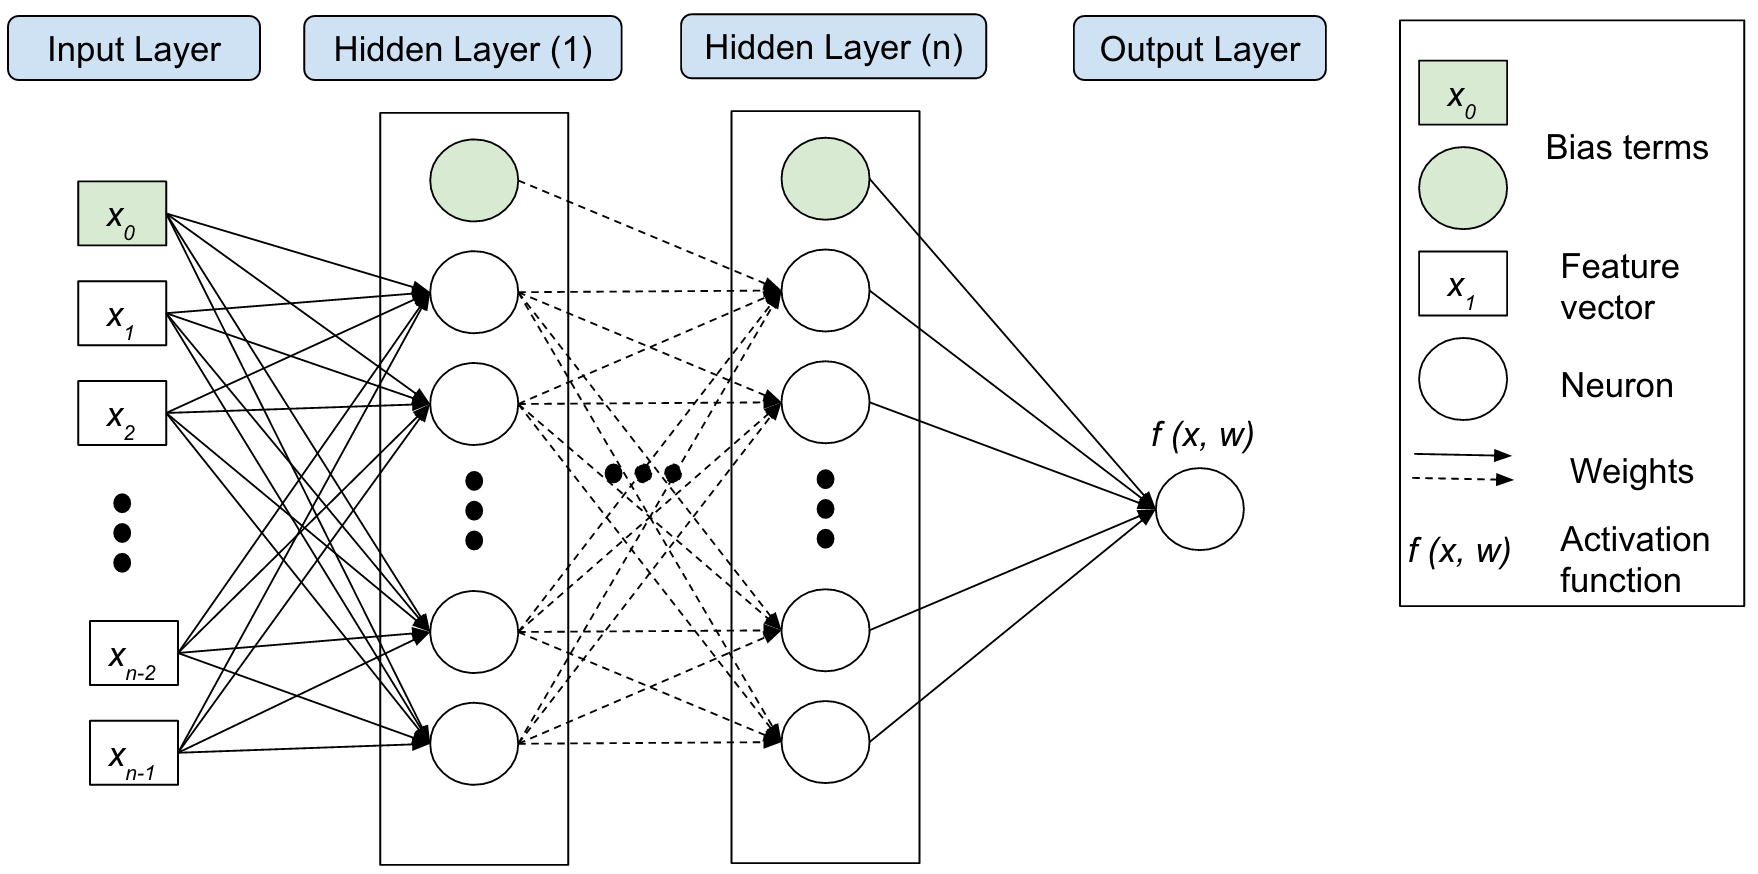
\includegraphics[width=0.7\linewidth]{figure_ann_architecture}
	\caption[ANN Architecture]{ANN Architecture}
	\label{fig:figure_ann_architecture}
\end{figure}

ANNs are excellent nonlinear modeling tools for approximating any non-linear relationships and finding patterns within the data (Jang et al., 1997) \cite{jang}. A \textit{feedforward neural network} is a nonliner function of its inputs, in which information flows from input nodes to output nodes. Each neuron in the network is a nonlinear combination of inputs $x_i$ weighted by the parameters $w_i$

Let $X$ be the training dataset with $n$ features, including the bias-term, then the output of a neuron is formulated as ($X \in R^{m \times n}, w \in R^{n}, y \in R ^{m}$):

\begin{equation}
f(y) = w^{T}  X 
\end{equation}

where $f$ is an activation function, a function that determines the actual output of the neuron. An activation function with nonlinear properties is important because of it's ability to discriminate relationships in the feature space and strongly influences the complexity and performance of a NN.  Duch et al., (1999) \cite{duch} performed an extensive research of activation functions (also referred as transfer functions with the domain of ANN) and Ozkan et al., (2003) \cite{ozkan} compared the performance of the following most common activation functions (Civco and Waug, 1994, Kaminsky et al., 1997) \cite{civco}, \cite{kaminsky}
\begin{enumerate}
	\item Linear: This is the identify activation function used for linear models
	\begin{equation}
	f(x) = x
	\end{equation}
	\item Sigmoid (Logisitc): Most commonly used activation function that has the range of $(0, 1)$
	\begin{equation}
	f(x) = \frac{1}{1 + e^{-x}}
	\end{equation}
	\item Tangent hyperbolic: Second most commonly used activation function after sigmoid and has the range of $(-1, +1)$
	\begin{equation}
	f(x) = \frac{1 - e^{2x}}{1 + e^{2x}}
	\end{equation}
\end{enumerate}









\subsection{Optimization}

\subsection{Train, Test and Validation Approaches}

\newpage\section{Results and Discussion}

\subsection{Data model and Exploratory Data Analysis}

\subsection{Results}

\newpage\section{Conclusions}

\newpage\section{References}

\begin{thebibliography}{100}  
\bibitem{adomavicius-2005} Adomavicius, G., \& Tuzhilin, A. (2005). Toward the next generation of recommender systems: A survey of the state-of-the-art and possible extensions. \textit{Knowledge and Data Engineering, IEEE Transactions on,17(6)}, 734-749.
\bibitem{adomavicius-2011} Adomavicius, G., \& Tuzhilin, A. (2011). Context-aware recommender systems. \textit{Recommender systems handbook}, 217-253.
\bibitem{amatriain} Amatriain, X. (2013). Big \& personal: data and models behind netflix recommendations. \textit{Proceedings of the 2nd International Workshop on Big Data, Streams and Heterogeneous Source Mining: Algorithms, Systems, Programming Models and Applications}. ACM.
\bibitem{amini} Amini, M., Nasiri, M., \& Afzali, M. (2014). Proposing a New Hybrid Approach in Movie Recommender System. \textit{International Journal of Computer Science and Information Security,12}(8), 40.
\bibitem{balabanovic} Balabanovic, Marko, and Yoav Shoham. Fab: content-based, collaborative recommendation. \textit{Communications of the ACM} 40.3 (1997), 66-72.
\bibitem{blattner} Blattner, M., \& Medo, M. (2012). Recommendation systems in the scope of opinion formation: a model. \textit{arXiv preprint arXiv:1206.3924}.
\bibitem{breese} Breese, J. S., Heckerman, D., \& Kadie, C. (1998). Empirical analysis of predictive algorithms for collaborative filtering. \textit{Proceedings of the Fourteenth conference on Uncertainty in artificial intelligence.} Morgan Kaufmann Publishers Inc.
\bibitem{burke} Burke, R. (2002). Hybrid recommender systems: Survey and experiments. \textit{User modeling and user-adapted interaction},12(4), 331-370.
\bibitem{carrillo} Carrillo, D., López, V. F., \& Moreno, M. N. (2013). Multi-label classification for recommender systems. \textit{Trends in Practical Applications of Agents and Multiagent Systems}, 181-188.
\bibitem{champiri} Champiri, Z. D., Shahamiri, S. R., \& Salim, S. S. B. (2015). A systematic review of scholar context-aware recommender systems. \textit{Expert Systems with Applications, 42}(3), 1743-1758.
\bibitem{chen} Chen, L., Chen, G., \& Wang, F. (2015). Recommender systems based on user reviews: the state of the art. \textit{User Modeling and User-Adapted Interaction, 25}(2), 99-154.
\bibitem{chen} Chen, Wei et al. "A hybrid recommendation algorithm adapted in e-learning environments. \textit{"World Wide Web} 17.2 (2014): 271-284.
\bibitem{cochocki} Cochocki, A., \& Unbehauen, R. (1993, June 1). \textit{Neural networks for optimization and signal processing}. John Wiley \& Sons, Inc.
\bibitem{edmunds} Edmunds, A., \& Morris, A. (2000). The problem of information overload in business organisations: a review of the literature. \textit{International journal of information management, 20}(1), 17-28.
\bibitem{felfernig} Felfernig, A., Isak, K., Szabo, K., \& Zachar, P. (2007). The VITA financial services sales support environment. \textit{PROCEEDINGS OF THE NATIONAL CONFERENCE ON ARTIFICIAL INTELLIGENCE}. Menlo Park, CA; Cambridge, MA; London; AAAI Press; MIT Press; 1999.
\bibitem{ge} Ge, X., Liu, J., Qi, Q., \& Chen, Z. (2011). A new prediction approach based on linear regression for collaborative filtering. \textit{Fuzzy Systems and Knowledge Discovery (FSKD), 2011 Eighth International Conference on}. IEEE.
\bibitem{gunawardana} Gunawardana, Asela, and Christopher Meek. A unified approach to building hybrid recommender systems. \textit{Proceedings of the third ACM conference on Recommender systems} 23 Oct. 2009: 117-124.
\bibitem{guo} Guo, S. (2011, October). \textit{Bayesian recommender systems: Models and Algorithms}. Australian National University.
\bibitem{gupta} Gupta, P., Goel, A., Lin, J., Sharma, A., Wang, D., \& Zadeh, R. (2013). Wtf: The who to follow service at twitter. \textit{Proceedings of the 22nd international conference on World Wide Web}. International World Wide Web Conferences Steering Committee.
\bibitem{hariri-2012} Hariri, N., Mobasher, B., \& Burke, R. (2012). Context-aware music recommendation based on latent topic sequential patterns. \textit{Proceedings of the sixth ACM conference on Recommender systems}. ACM.
\bibitem{hariri-2011} Hariri, N., Zheng, Y., Mobasher, B., \& Burke, R. (2011). Context-aware recommendation based on review mining. \textit{General Co-Chairs}, 27.
\bibitem{jannach} Jannach, D., Zanker, M., Felfernig, A., \& Friedrich, G. (2010, September 30). \textit{Recommender systems: an introduction}. Cambridge University Press.
\bibitem{kim} Kim, S., Pantel, P., Chklovski, T., \& Pennacchiotti, M. (2006). Automatically assessing review helpfulness. \textit{Proceedings of the 2006 Conference on empirical methods in natural language processing}. Association for Computational Linguistics.
\bibitem{lee} Lee, M., Choi, P., \& Woo, Y. (2002). A hybrid recommender system combining collaborative filtering with neural network. \textit{Adaptive Hypermedia and Adaptive Web-Based Systems}. Springer Berlin Heidelberg.
\bibitem{li} Li, M., Dias, B., El-Deredy, W., \& Lisboa, P. J. (2007). A probabilistic model for item-based recommender systems. \textit{Proceedings of the 2007 ACM conference on Recommender systems}. ACM.
\bibitem{linden} Linden, G., Smith, B., \& York, J. (2003). Amazon. com recommendations: Item-to-item collaborative filtering. \textit{Internet Computing, IEEE},7(1), 76-80.
\bibitem{mahalanobis} Mahalanobis, Prasanta Chandra (1936). "On the generalised distance in statistics" (PDF). \textit{Proceedings of the National Institute of Sciences of India}, 2(1): 49–55. Retrieved 2012-05-03.
\bibitem{mcculloch} McCulloch, W. S., \& Pitts, W. (1943). A logical calculus of the ideas immanent in nervous activity. \textit{The bulletin of mathematical biophysics}, 5(4), 115-133.
\bibitem{melville} Melville, Prem, Raymond J Mooney, and Ramadass Nagarajan. "Content-boosted collaborative filtering for improved recommendations." \textit{AAAI/IAAI} 28 Jul. 2002: 187-192.
\bibitem{miller g. a. 1956.txt} Miller G. A. 1956.txt,
\bibitem{milord} Milord, J. T., \& Perry, R. P. (1977). A Methodological Study of Overloadx. \textit{The Journal of General Psychology}, 97(1), 131-137.
\bibitem{moshfeghi} Moshfeghi, Y., Piwowarski, B., \& Jose, J. M. (2011). Handling data sparsity in collaborative filtering using emotion and semantic based features. \textit{Proceedings of the 34th international ACM SIGIR conference on Research and development in Information Retrieval}. ACM.
\bibitem{nanas} Nanas, N., Vavalis, M., \& Houstis, E. (2010). Personalised news and scientific literature aggregation. \textit{Information processing \& management, 46}(3), 268-283.
\bibitem{papagelis} Papagelis, M., Rousidis, I., Plexousakis, D., \& Theoharopoulos, E. (2005). Incremental collaborative filtering for highly-scalable recommendation algorithms. \textit{Foundations of Intelligent Systems}, 553-561.
\bibitem{pero} Pero, Š., \& Horváth, T. (2013). Opinion-driven matrix factorization for rating prediction. \textit{User Modeling, Adaptation, and Personalization}, 1-13.
\bibitem{pham} Pham, M. C., Cao, Y., Klamma, R., \& Jarke, M. (2011). A Clustering Approach for Collaborative Filtering Recommendation Using Social Network Analysis. \textit{J. UCS, 17}(4), 583-604.
\bibitem{raghavan} Raghavan, S., Gunasekar, S., \& Ghosh, J. (2012). Review quality aware collaborative filtering. \textit{Proceedings of the sixth ACM conference on Recommender systems}. ACM.
\bibitem{recommender systems.html} Recommender systems.html,
\bibitem{resnick} Resnick, P., \& Varian, H. R. (1997). Recommender systems. \textit{Communications of the ACM, 40}(3), 56-58.
\bibitem{ricci} Ricci, F., Rokach, L., \& Shapira, B. (2011). \textit{Introduction to recommender systems handbook Recommender systems handbook} (pp. 1-35). Springer US.
\bibitem{schein} Schein, A. I., Popescul, A., Ungar, L. H., \& Pennock, D. M. (2002). Methods and metrics for cold-start recommendations. \textit{Proceedings of the 25th annual international ACM SIGIR conference on Research and development in information retrieval}. ACM.
\bibitem{simon h. a. 1979.txt} Simon H. A. 1979.txt,
\bibitem{sorensen} Sorensen, S. (2012). Accuracy of Similarity Measures in Recommender Systems.
\bibitem{speier} Speier, C., Valacich, J. S., \& Vessey, I. (1999). The influence of task interruption on individual decision making: An information overload perspective. \textit{Decision Sciences, 30}(2), 337-360.
\bibitem{tu} Tu, J. V. (1996). Advantages and disadvantages of using artificial neural networks versus logistic regression for predicting medical outcomes. \textit{Journal of clinical epidemiology, 49}(11), 1225-1231.
\bibitem{vickery} Vickery, A., \& Vickery, B. C. (2004). \textit{Information science in theory and practice}. Walter de Gruyter.
\bibitem{wu} Wu, M., Chang, C., \& Liu, R. (2014). Integrating content-based filtering with collaborative filtering using co-clustering with augmented matrices. \textit{Expert Systems with Applications, 41}(6), 2754-2761.
\bibitem{zhang-narayan} Zhang, K., Narayanan, R., \& Choudhary, A. N. (2010). Voice of the Customers: Mining Online Customer Reviews for Product Feature-based Ranking. \textit{WOSN,10}, 11-11.
\bibitem{zhang-iyengar} Zhang, T., \& Iyengar, V. S. (2002). Recommender systems using linear classifiers. \textit{The Journal of Machine Learning Research}, 2, 313-334.
\bibitem{zheng} Zheng, Y. (2014). Semi-supervised context-aware matrix factorization: using contexts in a way of latent factors. \textit{Proceedings of the 29th Annual ACM Symposium on Applied Computing}. ACM.
\bibitem{marsland} Marsland, Stephen. \textit{Machine learning: an algorithmic perspective}. CRC press, 2015.
\bibitem{jang} J. -S. R. Jang, C.-T. Sun, and E. Mizutani, \textit{Neuro-Fuzzy and Soft Computing: A Computational Approach to Learning and Machine Intelligence}. Englewood Cliffs, NJ: Prentice-Hall, 1997.
\bibitem{ozkan} Özkan, Coşkun, and Filiz Sunar Erbek. "The comparison of activation functions for multispectral Landsat TM image classification." \textit{Photogrammetric Engineering \& Remote Sensing} 69.11 (2003): 1225-1234.
\bibitem{duch} Duch, Włodzisław, and Norbert Jankowski. "Survey of neural transfer functions." \textit{Neural Computing Surveys} 2.1 (1999): 163-212.
\bibitem{civco} Civco, D., and Y. Waug, 1994. Classification of multispectral, multitemporal, multisource spatial data using artificial neural networks, \textit{ASPRS/ACSM Annual Convention \& Exposition}, 25–28 April, Reno, Nevada (American Society for Photogrammetry and Remote Sensing, Bethesda, Maryland), pp. 123–133 
\bibitem{kaminsky} Kaminsky, E.J., H. Barad, and W. Brown, 1997. Textural neural network and version space classifiers for remote sensing, \textit{International Journal of Remote Sensing}, 18(4):741–762.

\end{thebibliography} 

\begin{flushleft}

\end{flushleft}

\bigskip
\end{document}
